\documentclass[border=2mm]{standalone}
\usepackage{tikz}
\usetikzlibrary{shapes.gates.logic.US}
\usetikzlibrary{circuits.ee.IEC}
\begin{document}
    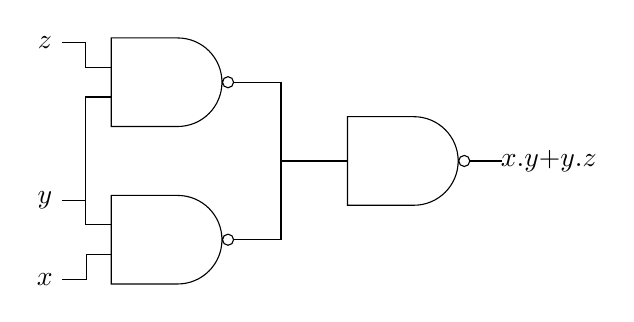
\begin{tikzpicture}[ circuit symbol wires]
    \node (x) at (0,0) {$x$};
    \node (y) at (0,1) {$y$};
    \node (z) at (0,3) {$z$};
    \node[nand gate US, minimum size=32pt, draw] at (1.5,0.5) (And) {};
    \node[nand gate US, minimum size=32pt, draw] at (1.5,2.5) (And1) {};
    \node[nand gate US, minimum size=32pt, draw] at (4.5,1.5) (And2) {};
    \draw (x.east) - ++(right:3mm) |- (And.input 2);
    \draw (y.east) - ++(right:3mm) |- (And.input 1);
    \draw (z.east) - ++(right:3mm) |- (And1.input 1);
    \draw (y.east) - ++(right:3mm) |- (And1.input 2);
    \draw (3.85,1.5) -- (3,1.5);
    \draw (3,0.5) -- (3,2.5);
    \draw (And.output) -- ($(And) + (1.5,0)$);
    \draw (And1.output) -- ($(And) + (1.5,2)$);
    \node (z) at ($(And2) + (1.9,0)$) {$x. y$+$y .z$};
    \draw (5.4,1.5) -- (5.8,1.5);
    \end{tikzpicture}
\end{document}
